% Created by tikzDevice version 0.12.4 on 2023-05-08 10:32:53
% !TEX encoding = UTF-8 Unicode
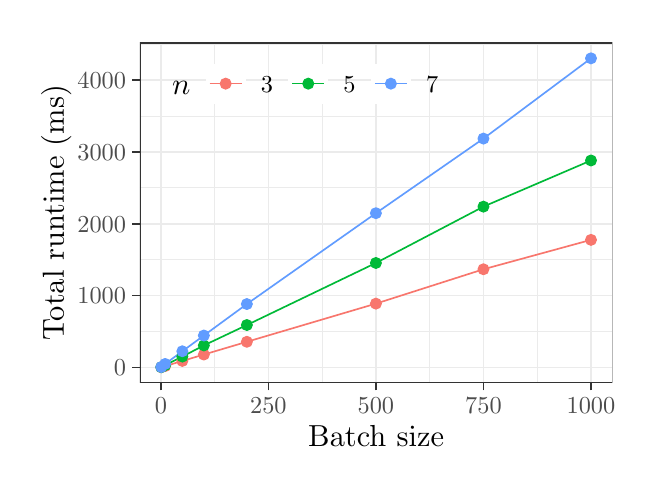
\begin{tikzpicture}[x=1pt,y=1pt]
\definecolor{fillColor}{RGB}{255,255,255}
\path[use as bounding box,fill=fillColor,fill opacity=0.00] (0,0) rectangle (216.81,158.99);
\begin{scope}
\path[clip] (  0.00,  0.00) rectangle (216.81,158.99);
\definecolor{drawColor}{RGB}{255,255,255}
\definecolor{fillColor}{RGB}{255,255,255}

\path[draw=drawColor,line width= 0.6pt,line join=round,line cap=round,fill=fillColor] (  0.00,  0.00) rectangle (216.81,158.99);
\end{scope}
\begin{scope}
\path[clip] ( 40.51, 30.69) rectangle (211.31,153.49);
\definecolor{fillColor}{RGB}{255,255,255}

\path[fill=fillColor] ( 40.51, 30.69) rectangle (211.31,153.49);
\definecolor{drawColor}{gray}{0.92}

\path[draw=drawColor,line width= 0.3pt,line join=round] ( 40.51, 49.19) --
	(211.31, 49.19);

\path[draw=drawColor,line width= 0.3pt,line join=round] ( 40.51, 75.15) --
	(211.31, 75.15);

\path[draw=drawColor,line width= 0.3pt,line join=round] ( 40.51,101.11) --
	(211.31,101.11);

\path[draw=drawColor,line width= 0.3pt,line join=round] ( 40.51,127.08) --
	(211.31,127.08);

\path[draw=drawColor,line width= 0.3pt,line join=round] ( 40.51,153.04) --
	(211.31,153.04);

\path[draw=drawColor,line width= 0.3pt,line join=round] ( 67.55, 30.69) --
	( 67.55,153.49);

\path[draw=drawColor,line width= 0.3pt,line join=round] (106.40, 30.69) --
	(106.40,153.49);

\path[draw=drawColor,line width= 0.3pt,line join=round] (145.26, 30.69) --
	(145.26,153.49);

\path[draw=drawColor,line width= 0.3pt,line join=round] (184.12, 30.69) --
	(184.12,153.49);

\path[draw=drawColor,line width= 0.6pt,line join=round] ( 40.51, 36.21) --
	(211.31, 36.21);

\path[draw=drawColor,line width= 0.6pt,line join=round] ( 40.51, 62.17) --
	(211.31, 62.17);

\path[draw=drawColor,line width= 0.6pt,line join=round] ( 40.51, 88.13) --
	(211.31, 88.13);

\path[draw=drawColor,line width= 0.6pt,line join=round] ( 40.51,114.10) --
	(211.31,114.10);

\path[draw=drawColor,line width= 0.6pt,line join=round] ( 40.51,140.06) --
	(211.31,140.06);

\path[draw=drawColor,line width= 0.6pt,line join=round] ( 48.12, 30.69) --
	( 48.12,153.49);

\path[draw=drawColor,line width= 0.6pt,line join=round] ( 86.98, 30.69) --
	( 86.98,153.49);

\path[draw=drawColor,line width= 0.6pt,line join=round] (125.83, 30.69) --
	(125.83,153.49);

\path[draw=drawColor,line width= 0.6pt,line join=round] (164.69, 30.69) --
	(164.69,153.49);

\path[draw=drawColor,line width= 0.6pt,line join=round] (203.55, 30.69) --
	(203.55,153.49);
\definecolor{drawColor}{RGB}{248,118,109}

\path[draw=drawColor,line width= 0.6pt,line join=round] ( 48.27, 36.27) --
	( 49.67, 36.70) --
	( 55.89, 38.56) --
	( 63.66, 40.87) --
	( 79.20, 45.48) --
	(125.83, 59.27) --
	(164.69, 71.69) --
	(203.55, 82.31);
\definecolor{drawColor}{RGB}{0,186,56}

\path[draw=drawColor,line width= 0.6pt,line join=round] ( 48.27, 36.30) --
	( 49.67, 37.01) --
	( 55.89, 40.14) --
	( 63.66, 44.17) --
	( 79.20, 51.54) --
	(125.83, 73.96) --
	(164.69, 94.32) --
	(203.55,111.00);
\definecolor{drawColor}{RGB}{97,156,255}

\path[draw=drawColor,line width= 0.6pt,line join=round] ( 48.27, 36.36) --
	( 49.67, 37.48) --
	( 55.89, 42.06) --
	( 63.66, 47.75) --
	( 79.20, 59.12) --
	(125.83, 91.95) --
	(164.69,118.91) --
	(203.55,147.91);
\definecolor{drawColor}{RGB}{248,118,109}
\definecolor{fillColor}{RGB}{248,118,109}

\path[draw=drawColor,line width= 0.4pt,line join=round,line cap=round,fill=fillColor] ( 48.27, 36.27) circle (  1.96);

\path[draw=drawColor,line width= 0.4pt,line join=round,line cap=round,fill=fillColor] ( 49.67, 36.70) circle (  1.96);

\path[draw=drawColor,line width= 0.4pt,line join=round,line cap=round,fill=fillColor] ( 63.66, 40.87) circle (  1.96);

\path[draw=drawColor,line width= 0.4pt,line join=round,line cap=round,fill=fillColor] (203.55, 82.31) circle (  1.96);

\path[draw=drawColor,line width= 0.4pt,line join=round,line cap=round,fill=fillColor] ( 79.20, 45.48) circle (  1.96);

\path[draw=drawColor,line width= 0.4pt,line join=round,line cap=round,fill=fillColor] ( 55.89, 38.56) circle (  1.96);

\path[draw=drawColor,line width= 0.4pt,line join=round,line cap=round,fill=fillColor] (125.83, 59.27) circle (  1.96);

\path[draw=drawColor,line width= 0.4pt,line join=round,line cap=round,fill=fillColor] (164.69, 71.69) circle (  1.96);
\definecolor{drawColor}{RGB}{0,186,56}
\definecolor{fillColor}{RGB}{0,186,56}

\path[draw=drawColor,line width= 0.4pt,line join=round,line cap=round,fill=fillColor] ( 48.27, 36.30) circle (  1.96);

\path[draw=drawColor,line width= 0.4pt,line join=round,line cap=round,fill=fillColor] ( 49.67, 37.01) circle (  1.96);

\path[draw=drawColor,line width= 0.4pt,line join=round,line cap=round,fill=fillColor] ( 63.66, 44.17) circle (  1.96);

\path[draw=drawColor,line width= 0.4pt,line join=round,line cap=round,fill=fillColor] (203.55,111.00) circle (  1.96);

\path[draw=drawColor,line width= 0.4pt,line join=round,line cap=round,fill=fillColor] ( 79.20, 51.54) circle (  1.96);

\path[draw=drawColor,line width= 0.4pt,line join=round,line cap=round,fill=fillColor] ( 55.89, 40.14) circle (  1.96);

\path[draw=drawColor,line width= 0.4pt,line join=round,line cap=round,fill=fillColor] (125.83, 73.96) circle (  1.96);

\path[draw=drawColor,line width= 0.4pt,line join=round,line cap=round,fill=fillColor] (164.69, 94.32) circle (  1.96);
\definecolor{drawColor}{RGB}{97,156,255}
\definecolor{fillColor}{RGB}{97,156,255}

\path[draw=drawColor,line width= 0.4pt,line join=round,line cap=round,fill=fillColor] ( 48.27, 36.36) circle (  1.96);

\path[draw=drawColor,line width= 0.4pt,line join=round,line cap=round,fill=fillColor] ( 49.67, 37.48) circle (  1.96);

\path[draw=drawColor,line width= 0.4pt,line join=round,line cap=round,fill=fillColor] ( 63.66, 47.75) circle (  1.96);

\path[draw=drawColor,line width= 0.4pt,line join=round,line cap=round,fill=fillColor] (203.55,147.91) circle (  1.96);

\path[draw=drawColor,line width= 0.4pt,line join=round,line cap=round,fill=fillColor] ( 79.20, 59.12) circle (  1.96);

\path[draw=drawColor,line width= 0.4pt,line join=round,line cap=round,fill=fillColor] ( 55.89, 42.06) circle (  1.96);

\path[draw=drawColor,line width= 0.4pt,line join=round,line cap=round,fill=fillColor] (125.83, 91.95) circle (  1.96);

\path[draw=drawColor,line width= 0.4pt,line join=round,line cap=round,fill=fillColor] (164.69,118.91) circle (  1.96);
\definecolor{drawColor}{gray}{0.20}

\path[draw=drawColor,line width= 0.6pt,line join=round,line cap=round] ( 40.51, 30.69) rectangle (211.31,153.49);
\end{scope}
\begin{scope}
\path[clip] (  0.00,  0.00) rectangle (216.81,158.99);
\definecolor{drawColor}{gray}{0.30}

\node[text=drawColor,anchor=base east,inner sep=0pt, outer sep=0pt, scale=  0.88] at ( 35.56, 33.18) {0};

\node[text=drawColor,anchor=base east,inner sep=0pt, outer sep=0pt, scale=  0.88] at ( 35.56, 59.14) {1000};

\node[text=drawColor,anchor=base east,inner sep=0pt, outer sep=0pt, scale=  0.88] at ( 35.56, 85.10) {2000};

\node[text=drawColor,anchor=base east,inner sep=0pt, outer sep=0pt, scale=  0.88] at ( 35.56,111.07) {3000};

\node[text=drawColor,anchor=base east,inner sep=0pt, outer sep=0pt, scale=  0.88] at ( 35.56,137.03) {4000};
\end{scope}
\begin{scope}
\path[clip] (  0.00,  0.00) rectangle (216.81,158.99);
\definecolor{drawColor}{gray}{0.20}

\path[draw=drawColor,line width= 0.6pt,line join=round] ( 37.76, 36.21) --
	( 40.51, 36.21);

\path[draw=drawColor,line width= 0.6pt,line join=round] ( 37.76, 62.17) --
	( 40.51, 62.17);

\path[draw=drawColor,line width= 0.6pt,line join=round] ( 37.76, 88.13) --
	( 40.51, 88.13);

\path[draw=drawColor,line width= 0.6pt,line join=round] ( 37.76,114.10) --
	( 40.51,114.10);

\path[draw=drawColor,line width= 0.6pt,line join=round] ( 37.76,140.06) --
	( 40.51,140.06);
\end{scope}
\begin{scope}
\path[clip] (  0.00,  0.00) rectangle (216.81,158.99);
\definecolor{drawColor}{gray}{0.20}

\path[draw=drawColor,line width= 0.6pt,line join=round] ( 48.12, 27.94) --
	( 48.12, 30.69);

\path[draw=drawColor,line width= 0.6pt,line join=round] ( 86.98, 27.94) --
	( 86.98, 30.69);

\path[draw=drawColor,line width= 0.6pt,line join=round] (125.83, 27.94) --
	(125.83, 30.69);

\path[draw=drawColor,line width= 0.6pt,line join=round] (164.69, 27.94) --
	(164.69, 30.69);

\path[draw=drawColor,line width= 0.6pt,line join=round] (203.55, 27.94) --
	(203.55, 30.69);
\end{scope}
\begin{scope}
\path[clip] (  0.00,  0.00) rectangle (216.81,158.99);
\definecolor{drawColor}{gray}{0.30}

\node[text=drawColor,anchor=base,inner sep=0pt, outer sep=0pt, scale=  0.88] at ( 48.12, 19.68) {0};

\node[text=drawColor,anchor=base,inner sep=0pt, outer sep=0pt, scale=  0.88] at ( 86.98, 19.68) {250};

\node[text=drawColor,anchor=base,inner sep=0pt, outer sep=0pt, scale=  0.88] at (125.83, 19.68) {500};

\node[text=drawColor,anchor=base,inner sep=0pt, outer sep=0pt, scale=  0.88] at (164.69, 19.68) {750};

\node[text=drawColor,anchor=base,inner sep=0pt, outer sep=0pt, scale=  0.88] at (203.55, 19.68) {1000};
\end{scope}
\begin{scope}
\path[clip] (  0.00,  0.00) rectangle (216.81,158.99);
\definecolor{drawColor}{RGB}{0,0,0}

\node[text=drawColor,anchor=base,inner sep=0pt, outer sep=0pt, scale=  1.10] at (125.91,  7.64) {Batch size};
\end{scope}
\begin{scope}
\path[clip] (  0.00,  0.00) rectangle (216.81,158.99);
\definecolor{drawColor}{RGB}{0,0,0}

\node[text=drawColor,rotate= 90.00,anchor=base,inner sep=0pt, outer sep=0pt, scale=  1.10] at ( 13.08, 92.09) {Total runtime (ms)};
\end{scope}
\begin{scope}
\path[clip] (  0.00,  0.00) rectangle (216.81,158.99);
\definecolor{drawColor}{RGB}{0,0,0}

\node[text=drawColor,anchor=base west,inner sep=0pt, outer sep=0pt, scale=  1.10] at ( 52.21,134.97) {$n$};
\end{scope}
\begin{scope}
\path[clip] (  0.00,  0.00) rectangle (216.81,158.99);
\definecolor{fillColor}{RGB}{255,255,255}

\path[fill=fillColor] ( 64.31,131.53) rectangle ( 78.77,145.98);
\end{scope}
\begin{scope}
\path[clip] (  0.00,  0.00) rectangle (216.81,158.99);
\definecolor{drawColor}{RGB}{248,118,109}

\path[draw=drawColor,line width= 0.6pt,line join=round] ( 65.76,138.76) -- ( 77.32,138.76);
\end{scope}
\begin{scope}
\path[clip] (  0.00,  0.00) rectangle (216.81,158.99);
\definecolor{drawColor}{RGB}{248,118,109}
\definecolor{fillColor}{RGB}{248,118,109}

\path[draw=drawColor,line width= 0.4pt,line join=round,line cap=round,fill=fillColor] ( 71.54,138.76) circle (  1.96);
\end{scope}
\begin{scope}
\path[clip] (  0.00,  0.00) rectangle (216.81,158.99);
\definecolor{fillColor}{RGB}{255,255,255}

\path[fill=fillColor] ( 94.16,131.53) rectangle (108.62,145.98);
\end{scope}
\begin{scope}
\path[clip] (  0.00,  0.00) rectangle (216.81,158.99);
\definecolor{drawColor}{RGB}{0,186,56}

\path[draw=drawColor,line width= 0.6pt,line join=round] ( 95.61,138.76) -- (107.17,138.76);
\end{scope}
\begin{scope}
\path[clip] (  0.00,  0.00) rectangle (216.81,158.99);
\definecolor{drawColor}{RGB}{0,186,56}
\definecolor{fillColor}{RGB}{0,186,56}

\path[draw=drawColor,line width= 0.4pt,line join=round,line cap=round,fill=fillColor] (101.39,138.76) circle (  1.96);
\end{scope}
\begin{scope}
\path[clip] (  0.00,  0.00) rectangle (216.81,158.99);
\definecolor{fillColor}{RGB}{255,255,255}

\path[fill=fillColor] (124.02,131.53) rectangle (138.47,145.98);
\end{scope}
\begin{scope}
\path[clip] (  0.00,  0.00) rectangle (216.81,158.99);
\definecolor{drawColor}{RGB}{97,156,255}

\path[draw=drawColor,line width= 0.6pt,line join=round] (125.46,138.76) -- (137.03,138.76);
\end{scope}
\begin{scope}
\path[clip] (  0.00,  0.00) rectangle (216.81,158.99);
\definecolor{drawColor}{RGB}{97,156,255}
\definecolor{fillColor}{RGB}{97,156,255}

\path[draw=drawColor,line width= 0.4pt,line join=round,line cap=round,fill=fillColor] (131.24,138.76) circle (  1.96);
\end{scope}
\begin{scope}
\path[clip] (  0.00,  0.00) rectangle (216.81,158.99);
\definecolor{drawColor}{RGB}{0,0,0}

\node[text=drawColor,anchor=base west,inner sep=0pt, outer sep=0pt, scale=  0.88] at ( 84.27,135.73) {3};
\end{scope}
\begin{scope}
\path[clip] (  0.00,  0.00) rectangle (216.81,158.99);
\definecolor{drawColor}{RGB}{0,0,0}

\node[text=drawColor,anchor=base west,inner sep=0pt, outer sep=0pt, scale=  0.88] at (114.12,135.73) {5};
\end{scope}
\begin{scope}
\path[clip] (  0.00,  0.00) rectangle (216.81,158.99);
\definecolor{drawColor}{RGB}{0,0,0}

\node[text=drawColor,anchor=base west,inner sep=0pt, outer sep=0pt, scale=  0.88] at (143.97,135.73) {7};
\end{scope}
\end{tikzpicture}
